\documentclass{article}
\usepackage[bottom=2cm, right=1.5cm, left=1.5cm, top=2cm]{geometry}
\usepackage{amsmath}
\usepackage{amssymb}
\usepackage{amsthm}
\usepackage{enumitem}
\usepackage{exercise} % Exercises Style
\usepackage{graphicx}
\usepackage{caption}
\usepackage{environ}



% Enable Code
\usepackage{minted}
\let \extra T

\newcommand{\vect}[1]{\boldsymbol{#1}}
\DeclareMathOperator{\Tr}{Tr}
\DeclareMathOperator{\Cov}{Cov}
\DeclareMathOperator{\Var}{Var}
\DeclareMathOperator{\E}{E}

\usepackage{fancyhdr}
\newenvironment{solution}
  {\renewcommand\qedsymbol{$\blacksquare$}\begin{proof}[Solution]$ $}
  {\end{proof}}

\title{Solutions to Assignment }
\author{Rongfei Jin}
\begin{document}

\pagestyle{fancy}
\fancyhf{}%
\fancyhead[L]{\textbf{ \ Assignment }}
\fancyhead[R]{\textbf{Rongfei Jin}}
\fancyfoot[C]{\thepage}%
\maketitle

\section{Conceptual 1}
\begin{align*}
    \underset{a}{\arg\min} \Var (aX + (1-a)Y)
    &= \underset{a}{\arg\min} \Var (aX) + \Var ((1-a)Y) + 2\Cov(aX, (1-a)Y) \\
    &= \underset{a}{\arg\min} \left\{a^2\Var(X) + (1-a)^2\Var(Y) + 2a(1-a)\Cov(X, Y)\right\}
\end{align*}

We solve the above equation by taking the derivative with respect to $a$ and setting it to zero:
\[\frac{d}{da} \left[a^2\Var(X) + (1-a)^2\Var(Y) + 2a(1-a)\Cov(X, Y)\right] = 2a\Var(X) - 2(1-a)\Var(Y) + (2-4a)\Cov(X, Y)\]

\begin{align*}
    2a\Var(X) - 2\Var(Y) + 2a\Var(Y) + 2\Cov(X, Y) - 4a\Cov(X, Y) &= 0 \\
    2a(\Var(X) + \Var(Y) - 2\Cov(X, Y)) + 2\Cov(X, Y) - 2\Var(Y) &= 0 \\
    a &= \frac{\Var(Y) - \Cov(X, Y)}{\Var(X) + \Var(Y) - 2\Cov(X, Y)} \\
    a &= \frac{\sigma_Y^2 - \sigma_{XY}}{\sigma_X^2 + \sigma_Y^2 - 2\sigma_{XY}}
\end{align*}

\section{Conceptual 2}
\begin{enumerate}[label=(\alph*)]
\item \[\Pr(\text{first pick is not jth observation}) = \frac{\text{\# choices not jth observation}}{\text{\# all choices}} = \frac{n-1}{n}\]
\item Same as above, the probability is $\frac{n-1}{n}$ since the picks are independent.
\item \[\Pr(\text{all n picks are not jth observation}) = n\cdot \Pr(\text{first pick is not jth observation}) = (\frac{n-1}{n})^n = (1- \frac{1}{n})^n\]
\item If \(n=5\) then \(Pr(\text{jth observation in the resample}) = 1 - (\frac{4}{5})^5 \)
\item Similar to above, the probability is \(1 - (\frac{99}{100})^{100}\)
\item \(1- \frac{9999}{10000}^{10000}\)
\item The limit of the expression is \(1 - \frac{1}{e} \approx 0.632 \) and the plot confirms this.

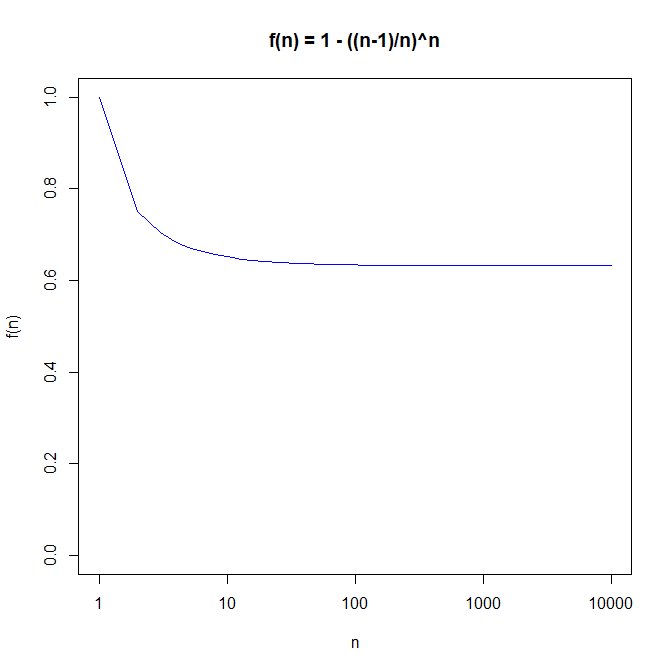
\includegraphics[scale=0.5]{q2-1.png}
\item The simulation result is 0.6337 which is very close to the theoretical result.

\end{enumerate}

\section{Additional 1}

When the error term is not normally-distributed, the estimates are not normally distributed. Thus inference on the estimates are not reliable unless the distribution of the error is known. However, for large sample sizes, the estimates are approximately normally distributed due to the Central Limit Theorem.

\newpage
\section {Additional 2}
\inputminted{r}{q4.r}

\begin{enumerate}[label=(\alph*)]
\item[(b)] The bootstrap confidence are very close to the standard confidence intervals.
\end{enumerate}
\newpage
\section {Additional 3}
\inputminted{r}{q5.r}


\begin{enumerate}[label=(\alph*)]
\item The OLS esimate lies within the 95 confidence interval of the bootstrapped data and the CIs are very close to each other.
\item The histogram of the bootstrapped are approximiately symmetric and normally distributed. The histogram supports the difference between the CI estimates. For the logMiles, the bootstrap CI is wider at the left tail and narrower at the right tail. For the logWeight, the bootstrap CI is wider at the right tail and narrower at the left tail.
\end{enumerate}

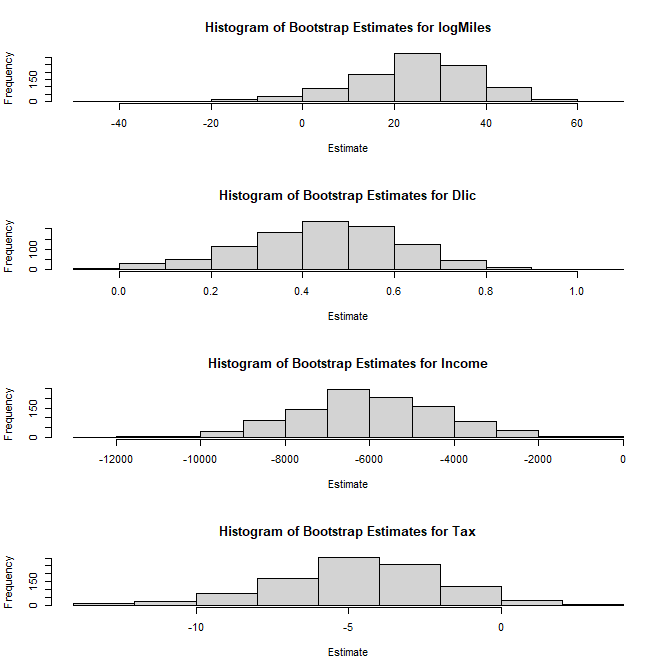
\includegraphics[scale=0.5]{q5.png}

\end{document}